\documentclass{article}

%\renewcommand{\thesection}{\Roman{section}} 
%\renewcommand{\thesubsection}{\thesection.\Roman{subsection}}
\usepackage{graphicx}
\graphicspath{ {images/} }

% Setting Margin for Report
\usepackage[margin=1.75in]{geometry}


%Begin Report
\begin{document}



\title{\textbf{Simulation Study: Classification Performance of Random Forest vs Logistic Regression}}
\author{Jacob Brionez, Kaitlin Kirasich, Bivin Sadler, Trace Smith}

\institute{$^1$Master of Science in Data Science \\ Southern Methodist University \\ Dallas, Texas USA \\\date{\today}

\begin{document}
\[\maketitle

\begin{abstract} 
Classification and regression performance of statistical based learning algorithms has been widely studied for certain types of data or applications. In supervised learning, the objective of the learning algorithm is to learn a set of parameter estimates such that the loss function is minimized by deploying optimization techniques. Numerous machine learning algorithms currently exist that are utilized for predictive analytics in various domains such as ensemble learners, support vector machines, and neural networks. Selecting a learning algorithm to implement for a particular application on the basis of performance still remains an ad-hoc process using fundamental benchmarks such as evaluating a classifier’s overall loss function, area under the curve (AUC) score, specificity, and sensitivity values. The basis of this work is to present a methodology for evaluating and determine the circumstances in which one machine learning algorithm may perform better than another under various simulated data structures benchmarked by classification performance statistics.
\end{abstract}

\section{Introduction}
The success of machine learning models is attributed to identifying predictor variables that best approximates the functional relationship between the input features and the response variable. It is well known that irrelevant features included in a dataset during the training process can lead to rising computational complexity in addition to overfitting, which can present misleading performance metrics as the model will not generalize to the out-of-sample dataset. This work is aimed at assisting a Data Scientist in evaluating which machine learning model to deploy for a variety of dataset types in specific scenarios. This study consists of investigating the performance between logistic regression and random forest models for datasets comprised of explanatory variables with varying degrees of correlation in addition to a series of noisy variables which pose no direct relationship with the response. This interactive tool will allow users the flexibility to simulate training datasets that have either a large or small number of predictor variables as well as any number of observations. Given the simulated dataset output, the tool will evaluate logistic regression and random forest on the Type I error, failure to reject noise variables by utilizing forward, backward, or stepwise selection criteria, and the highest prediction accuracy and AUC score. One possible application of the analytical tool, developed in R Shiny, would be to simulate a particular data structure that resembles a real-world dataset in order to draw inferences as to which model performs better under certain scenarios and yields the highest precision and accuracy on feature retention rate. For instance, one particular question examines whether logistic regression or random forest achieves a better performance metric with multiple covariates simulated with various sample sizes. (TODO: move to conclusion) While developing the model recommendation pipeline, this work can be expanded beyond logistic regression and random forest models, the concept is aimed at providing Data Scientists the tools necessary to evaluate the expected model performance on simulated data before selecting a model to deploy in a real-world application.


\section{Problem}

Within the past few years, the use of predictive analytics has become more prevalent in everyday decision making across many industries. Despite the vast amount of data rapidly being collected, the advancements in big data processing capabilities and decrease in storage expenses, model selection remains a persistent challenge for Data Scientists. When it comes to selecting between the random forest and logistic regression models, the optimal model can vary given the underlying structure of the data.  Thus, investigating conditions in which prompts one learning algorithm to outperform another is one of the motivators for this work.  

Numerous studies have been published that compare random forest and logistic regression algorithms, but most research experiments consisted of either a single dataset or multiple datasets from the same source. In these scenarios, sometimes logistic regression performed better while in other cases random forest performed better.  For example, one experiment used several neuropsychological tests to predict dementia.  This stated that with respect to specificity and overall classification accuracy, random forest and linear discriminant analysis rank first among all the classifiers including logistic regression (Guerreiro, 2011).  Contrastingly, in another article analyzing Twitter tweets surrounding the 2016 United States election, it was found that when PCA is applied to tweets, logistic regression provides better results than random forest (Beğenilmiş, 2017).  The type of data and data sources used in the studies above are drastically different from each other and each algorithm performs differently due to the type of data it was using to try to classify. Our project aims to provide a method to evaluate random forest and logistic regression models for a variety of data conditions.

While we focus our work on model selection, another important piece to selecting the right model for your dataset is making sure the input features are selected appropriately.  Criteria for identifying significant input features in a model varies between domains and datasets at hand. Automated feature selection has widely been studied, ranging from computer vision, classification, and regression types of problems. Zoran et al proposed a purposeful selection of covariates algorithm that automates feature selection by iteratively refitting the model by either adding or removing variables to verify if the model contains statistically significant predictors or confounders with a maximum p-value of 0.25 (Zoran, 2008). Traditionally, the significance threshold is 0.05; although there is only a 5\% chance of a Type I error, variables of importance could be misclassified. In this simulation study, the purposeful selection method evaluates significance at the 0.10 level and if the parameter estimate value alters 20\% compared to the full model, then there is evidence the excluded variable was of importance and is therefore added back to the model (Zoran, 2008). The novel method was applied on two different simulated datasets and was compared with stepwise, forward, and backward selection as a benchmark for the conclusion.

Logistic regression was the model of choice for the two simulation experiments performed by Zoran et al, consisting of six total explanatory variables and six different sample sizes. The first study consisted of only three significant variables of equal parameter estimates and three non-significant predictors. Secondly, the simulation was altered slightly to contain two significant variables, one confounder which is dependent on X1, and three non-significant variables with parameter estimate of zero, respectively. For both simulation cases, the average retention rate for 1000 iterations correctly identified variables increased with respect to an increase in sample size (Zoran, 2008). 

Another automated feature selection tool we found is TPOT. TPOT is a recently developed tool built in Python which optimizes machine learning pipelines via genetic programming with the goal of maximizing classification accuracy on any supervised classification problems (Olsen, 2016). Similar to what a content management system is to a website where anyone who has no knowledge of web development can edit a website, TPOT does the same for machine learning.  The tool takes in a dataset and picks out the best features to generate an optimized model for prediction and classification (Olsen, 2016).  Another feature engineering tool discovered is called One Button Machine, or OneBM, which automates the extraction of useful features from relational databases (Lam, 2017). To validate the model results obtained from the developed application presented in this work, one method would consist of utilizing TPOT or OneBM to compare variable selection and model performance of both logistic regression and random forest.

\section{Machine Learning Models}

\subsection{Random Forest}

Random forest is an ensemble based learner which is comprised of 'n' collection of de-correlated trees (Hastie, 2009). Built off the idea of bootstrap aggregation which with a method for resampling with replacement in order to reduce variance, random forest uses multiple trees to average (regression) or computes majority votes (classification) in the terminal leaf nodes when making a prediction. Decision trees themselves are prone to overfitting noise in a training set which ultimately leads to results with high variance. In other words, this means the model could accurately predict the same data it was trained on but may not possess the same performance on datasets without the similar patterns and variations in the training set. As previously stated, random forest solves this overfitting of data by averaging multiple decision trees trained on different parts of the training set. 


\subsection{Logistic Regression}

Linear models are composed of one or multiple independent variables that describes a relationship to a dependent response variable. Mapping qualitative or quantitative input features to a target variable that is attempted to being predicted such as financial, biological, or sociological data is known as supervised learning in machine learning terminology if the labels are known.  One of the most common utilized linear statistical models for discriminant analysis is logistic Regression.

\begin{equation}
\pi_{i} = \beta_{0} + \beta_{1}X_{1} + .....\beta_{n}X_{n}
\end{equation}

Simplicity and interoperability of logistic Regression can occasionally lead to outperforming other sophisticated nonlinear models such as ensemble learners or support vector machines. However, in the event the response variable is drawn from a small sample size, then linear regression models become insufficient and performs poorly for binary responses A number of learning algorithms could be applied to modeling binary classification data types, however the focal point of this work is to examine one linear model, logistic regression. 
 
Unlike the response variable for Linear Regression which is quantitative, the target variable for logistic regression is the posterior probability of being classified in the ith group of a binary or multi-class response (Hastie, 2009). Logistic regression makes several assumptions such as independence, responses (logits) at every level of a subpopulation of the explanatory variable are normally distributed, and constant variance between the responses and all values of the explanatory variable. Intuitively, a transformation to the response variable is applied to yield a continuous probability distribution over the output classes bounded between 0 and 1; this transformation is called to “logistic” or “sigmoid” function where ‘z’ corresponds to log odds divided by the logit (Ng, 2008).

\begin{equation}
\sigma(Z) = \frac{1}{1+\exp^{-z}}
\end{equation}


\begin{figure}
\centering
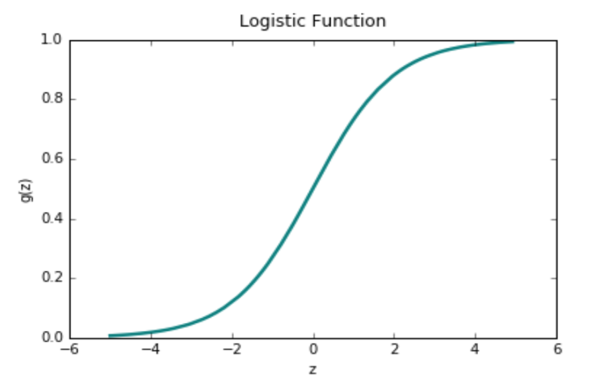
\includegraphics[scale=1.0]{sigmoid.png}
\caption{Log of Odds Function}
\end{figure}

For a binary response, the logistic regression model can be expressed by summing over the linear combinations of input features and a corresponding weight plus a bias terms for each instance as shown below in equation (3) and (4).

\begin{equation}
p(y^{(i)} = 1 | x^{(i)},w) = 1-  \frac{1}{1+\exp^{(w^{T}x^{(i)}+b)}}
\end{equation}
\begin{equation}
p(y^{(i)} = 0 | x^{(i)},w) = 1-  \frac{1}{1+\exp^{(w^{T}x^{(i)}+b)}}
\end{equation}


The objective is to find a set of weights such that the negative log likelihood is minimized over the defined training set using optimization techniques such as gradient descent or stochastic gradient descent [3]. Minimizing the negative log likelihood also means maximizing the likelihood or probability the parameter estimate pi of selecting the correct class. The loss function that measures the difference between the ground truth label and the predicted class label is referred to as the cross-entropy. If the prediction is very close to the ground truth label, the loss value will be low. Alternatively, if the prediction is far from the true label, the resulting log loss will be higher.

\begin{equation}
J(\theta) = -\frac{1}{m}\sum p_{i}log(y_{i}) + (1-p_{i})log(1-y_{i})
\end{equation}

\section{R Shinny Analytical Tool}

To conduct the statistical analysis, an interactive web application was developed which allows end users to rapidly generate simulated datasets with minimal overhead. Obtaining data from various input streams and performing cleaning transformations can be a lengthy process and create bottlenecks in the process of rapid deploying machine learning models. However, a combination of prior domain knowledge and familiarity of characteristics and patterns within a particular dataset can allow Data Scientists to synthetically generate data that closely resembles a real-world dataset as a proxy for evaluating performances of machine learning models.  Built under the R Shiny framework and utilizing the R programming language, this application allows for Data Scientist to easily simulate dataset and evaluate models without maintaining or configuring servers, security, and hardware as the application is run and maintained in a cloud environment. 

The application requires several input arguments to be configured prior to generating a dataset of an arbitrary length. Once specifying the number of explanatory variables, weighting factors of the explanatory feature coefficients, number of noise variables, distributions (e.g. gamma or normal), an open source package, \textit{simstudy}, is then called to create a dataset with the corresponding defined parameters. As a constraint for the analysis, the mean is set equal to zero, while the variance is altering in magnitude, ranging between 0.50 and 5.0. Furthermore, given this study is focused on analyzing classification, only binary response variables are considered. The response variable is a function of the log odds for the specified beta coefficients and noise variables. 


\begin{figure}
\centering
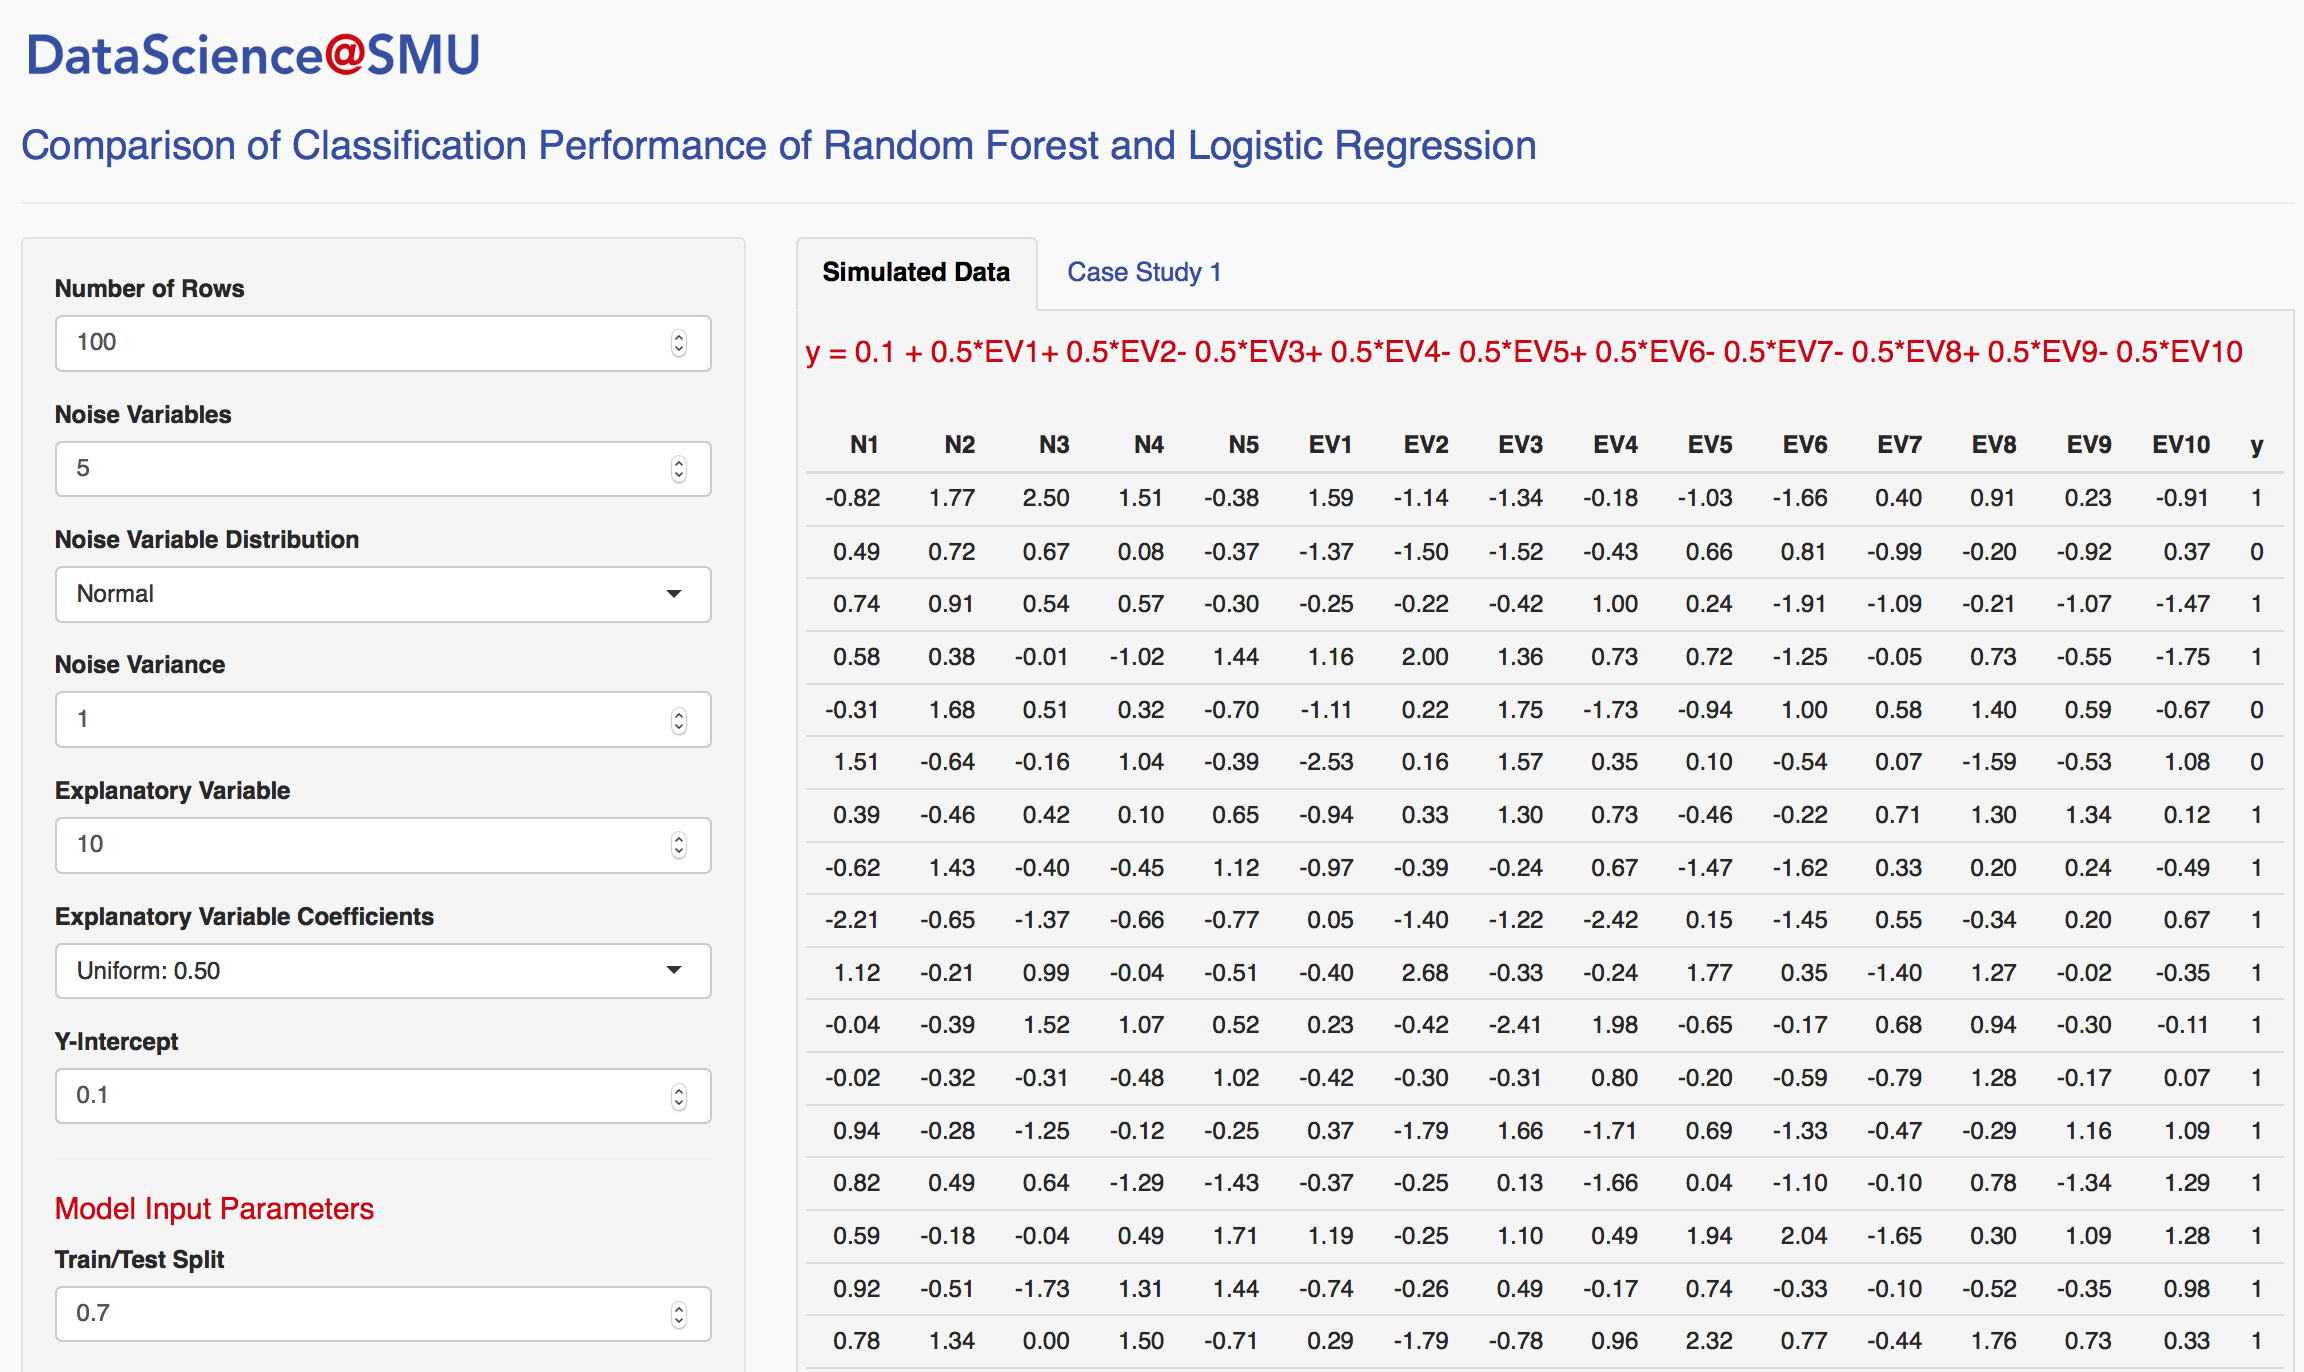
\includegraphics[scale=0.30]{simulation.png}
\caption{R Shinny Application - Data Simulator}
\end{figure}


\section{Criteria for Model Comparison}

The criteria we use to compare a machine learning algorithm’s model selection performance are type 1 errors, type 2 errors, and AIC.  When comparing the machine learning model’s accuracy we use the misclassification rates and AUC.  Type 1 errors are defined as a false positive finding.  We use this when looking at what variables each model selects.  A type 1 error is when a machine learning algorithm finds a model that includes noise variables thinking it is an explanatory variable.  Type 2 errors are the false negative findings that occur when our machine learning algorithm chooses a model that leaves out a true explanatory variable. The Akaike information criterion, or AIC, is an estimator of quality in model selection and is used when comparing the same type of model under different conditions.  It comes from information theory as estimate of the relative information lost when a given model is used to represent the process that generated the data.  It cannot define the quality of one model, but it can define the quality relative to another model.

After selecting a model from each algorithm and training it, misclassification rates between the two models on the testing set are compared. The true positive rate (sensitivity), true negative rate (specificity), false positive rate, and false negative rate are also benchmarked. True positive rate and sensitivity are calculated as the portion of positives or successes that are correctly identified.  False positive rate is the portion that was incorrectly identified as positive or success but is actually negative.  True negative rate and specificity are defined as the portion of negatives that are correctly identified.  The false negative rate would be the portion of incorrectly identified negatives.  Depending on your application, you may care about incorrectly classifying a positive more than incorrectly classifying a negative.  For example, when dealing with anything medical or health related, one is likely more focused on correctly identifying a positive and minimizing the false negative rate.  When dealing with automated event or airport security, it may be okay to have a higher false negative rate because it may be cheap and non-life threatening to confirm the automated alert.

These data points can be graphically represented using the receiver operating characteristic curve or ROC curve.  The ROC curve is a graph with the x axis from 0 to 1 of the false positive rate, and the y axis from 0 to 1 of the true positive rate at various threshold settings.  A perfect predictor would have a false positive rate of 0 and a true positive rate of 1.  When graphed over a series of thresholds, we would want to look at the area under the curve, or AUC.  The higher the AUC, the better our model performs.  

\section{Results}

In this analysis, two controlled case studies were conducted and results contrasted between both classifiers, random forest and logistic regression. Case Study 1 consisted of simulating a dataset with 10 observations, 5 noise variables, and 10 explanatory variables, respectively. For the explanatory variables, a random sample is drawn from a gaussian distribution with a mean of zero and standard deviation of unity. The parameter estimates for the explanatory and noise variables are weighted such that the response variable is a function of a series of features with equal coefficients of 0.50.  Once generating the data, the effects of training a random forest and logistic regression model with respect to varying levels of variation in the noise variables was investigated. For this specific simulation study, each model was simulated 10 times with a different dataset simulated of the same input parameters for differing levels of standard deviation for the noise ranging between 0.50 and 5.0.

Thresholding the variance in increments of 0.50, the 100 simulations’ misclassification rates are summarized in Figure X.  A plot of misclassification rates for each model in also shown in Figure X.  Given the small sample size of 100 data points, inconsistency and non-stationary levels of accuracies are observed and thus does not provide conclusive evidence in model recommendation under these conditions. To address these concerns, the number of iterations is increased to100 simulations and the previously described process is repeated. Likewise,  similar to the case of 10 simulations, logistic regression performs better when classifying positives events correctly. On the other hand, the overall testing accuracy is still very similar for both models. The hypothesis would expect to see a point in the variance which one model would start to outperform the other. Finally, the same process was repeated, however for 1000 simulations. Similar to before, logistic regression did a better job of correctly classifying positives in contrast to random forest.  However, there is no conclusive indication of when random forest or logistic regression will out perform the other in accuracy over varying levels of variance of the noise variables.

\section{Ethics}

As presented in this work, an analytical tool generates synthetic data in an effort to evaluate and compare logistic regression and random forest models. Therefore, as the data is a product of a simulator, this does not provide any legal violations or security concerns. It should be clearly stated that the users should only consider the tool for educational purposes only as this application is still in the development phase. Any decisions drawn from the tool are not endorsed by the authors of this paper.   

\section{Conclusion}

(In progress...)
Based on the simulation study conducted in this work, logistic regression correctly classifying true positives better as opposed to random forest. Random forest and logistic regression have similar accuracy over varying levels of variance for noise variables. The expectation that there is an indication where logistic regression or random forest would perform better but there is no indication of this at this point.  


\newpage
\begin{thebibliography}{9}

\bibitem{einstein} 
Guerreiro, Manuela; Maroco, João; de Mendonça, Alexandre; Rodrigues, Ana; Santana, Isabel; Silva, Dina. Data mining methods in the prediction of Dementia: A real-data comparison of the accuracy, sensitivity and specificity of linear discriminant analysis, logistic regression, neural networks, support vector machines, classification trees and random forests. BMC Research Notes20114:299. https://doi.org/10.1186/1756-0500-4-299.

\bibitem{einstein} 
Beğenilmiş, Erdem; Üsküdarlı, Suzan.  Organized Behavior Classification of Tweet Sets using Supervised Learning Methods. eprint arXiv:1711.10720. 11/2017.

\bibitem{einstein} 
Thanh Lam, Hoang; Thiebaut, Johann-Michael; Sinn, Mathieu; Chen, Bei; Mai, Tiep; Alkan, Oznur.  One button machine for automating feature engineering in relational databases. eprint arXiv:1706.00327. 06/2017.

\bibitem{einstein} 
Olson, Randal S.; Moore, Jason H.  Identifying and Harnessing the Building Blocks of Machine Learning Pipelines for Sensible Initialization of a Data Science Automation Tool. eprint arXiv:1607.08878. 07/2016. 

\bibitem{einstein} 
Graham Dunn. (2007) Regression Models for Method Comparison Data. Journal of Biopharmaceutical Statistics 17:4, pages 739-756

\bibitem{einstein} 
Hastie, T., Tibshirani, R., Friedman, J. (2009). The elements of statistical learning: data mining, inference and prediction. Springer. 

\bibitem{einstein} 
Andrew Ng. CS229 Lecture Notes. Stanford University. 2012

\bibitem{einstein} 
Zoran Bursac, C Heath Gauss, David Keith Williams, David W Hosmer: Purposeful Selection of Variables in Logistic Regression. Source Code for Biology and Medicine. 2008

\end{thebibliography}

\newpage
\section{Appendix}

\begin{figure}
\centering
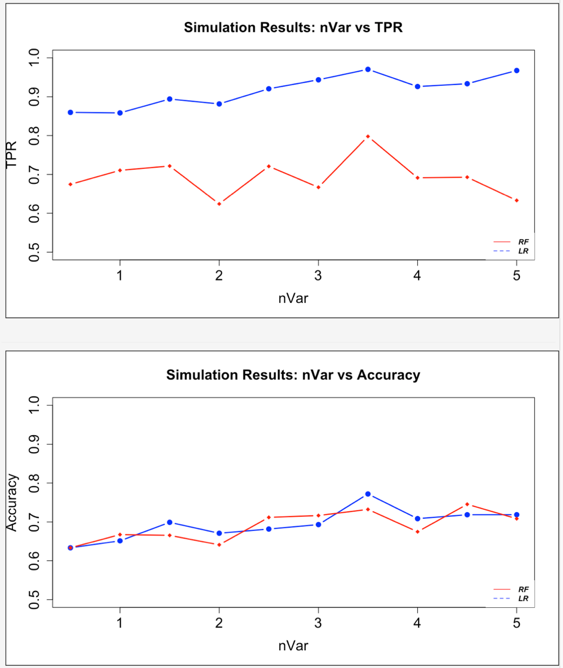
\includegraphics[scale=1.15]{simulation_results_case1_10plot.png}
\caption{Simulation Case Study 1: 10 Simulations}
\end{figure}

\begin{figure}
\centering
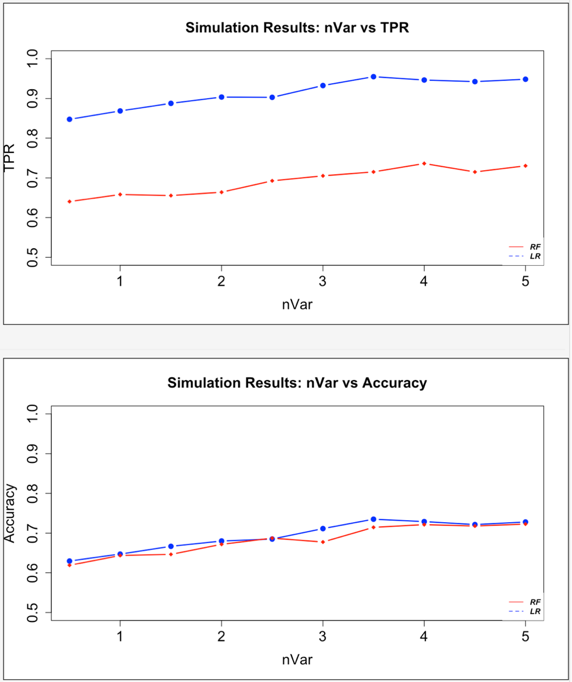
\includegraphics[scale=1.15]{simulation_results_case1_100plot.png}
\caption{Simulation Case Study 1: 100 Simulations}
\end{figure}

\begin{figure}
\centering
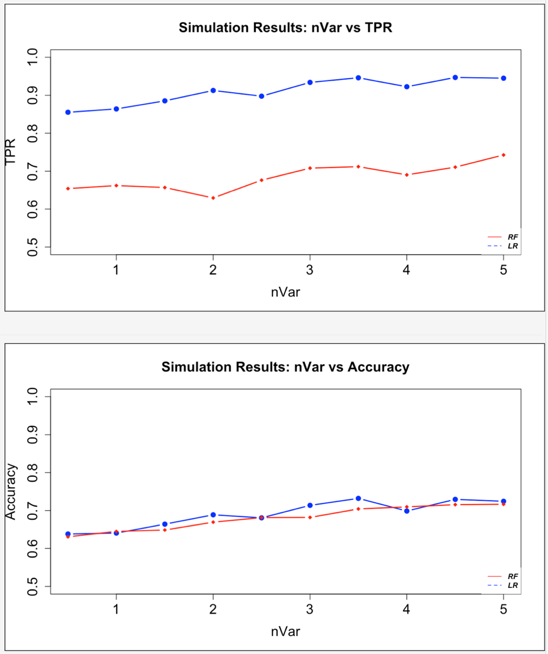
\includegraphics[scale=1.15]{simulation_results_case1_1000plot.png}
\caption{Simulation Case Study 1: 100 Simulations}
\end{figure}

\begin{figure}
\centering
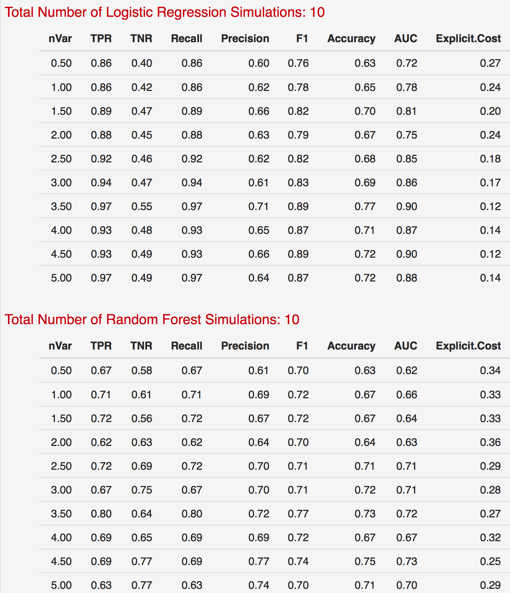
\includegraphics[scale=1.0]{simulation_results_case1_10sum.png}
\caption{Simulation Case Study 1: 10 Simulations}
\end{figure}

\begin{figure}
\centering
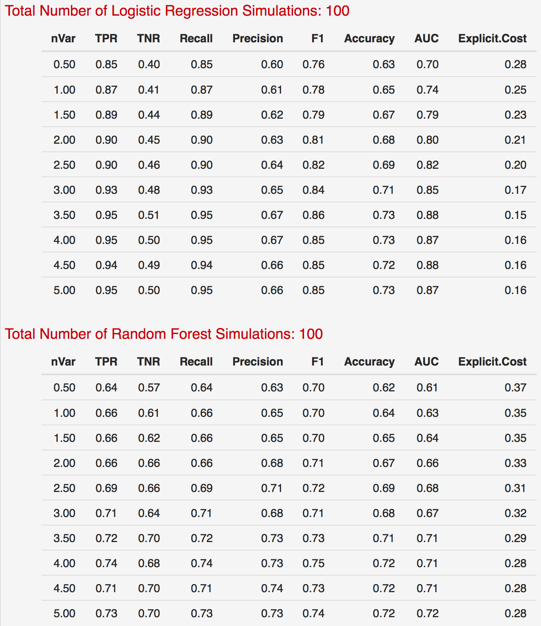
\includegraphics[scale=1.0]{simulation_results_case1_100sum.png}
\caption{Simulation Case Study 1: 100 Simulations}
\end{figure}

\begin{figure}
\centering
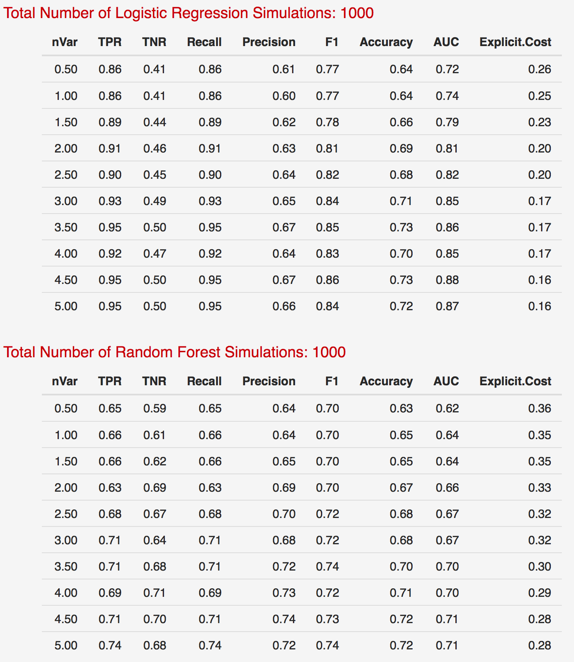
\includegraphics[scale=1.0]{simulation_results_case1_1000sum.png}
\caption{Simulation Case Study 1: 100 Simulations}
\end{figure}



\]
\end{document}